\documentclass[
	parskip=half,10pt,
	numbers= noenddot, % enddot -> Ebenen mit Punkt abschließen -> 1.1., noenddot -> ohne Punkt
	toc=flat, % TOC in Tabellenform (bei langen Überschrtiften verwenden)
	oneside,
	twocolumn,
	]{scrartcl}



\usepackage[T1]{fontenc} % verwende Type 1 - Zeichensatz
\usepackage{libertine}
\usepackage[scaled=0.78]{beramono} %Schreibmaschinenschrift
\usepackage{microtype}
\usepackage[utf8]{inputenc}
\usepackage[english]{babel} % internationale Sprachunterstützung



\usepackage{amsmath}
\usepackage{amssymb}
\usepackage{amsthm}
\usepackage{tabularx}
\usepackage{booktabs}
\usepackage{longtable}
\usepackage{rotating} % Rotationen, Reflexionen, ...
\usepackage{multido} % Wiederholungen
\usepackage{wrapfig}
\usepackage{todonotes}
\usepackage{siunitx} %\si units
\usepackage{units}
\usepackage{icomma} %keine Leerzeichen nach Komma im mathmode
\usepackage[numbers,sort]{natbib}
\usepackage{babelbib} %deutsche bibliographie
\usepackage{multirow}
\usepackage{rotating}
\usepackage{url}

\usepackage{tikz}
\usepackage{float}
\usepackage{pgfplots}
%\pgfplotsset{compat=1.8}
\usepackage{caption}
\usepackage{graphicx}
\usepackage{subcaption} %für subfigures
\captionsetup{labelfont={bf,sf},format = plain, textfont=sf}
%\usepackage{asymptote}
\usepackage{ragged2e}
\usepackage[bottom]{footmisc}
\usepackage{csquotes} %Anführungszeichen
\usepackage[ngerman]{varioref} % Zum komfortablen Verlinken



\usepackage{geometry}
\geometry{a4paper,lmargin=2.5cm, rmargin=2.5cm, tmargin=2.5cm, bmargin=3cm, marginparwidth=3cm, marginparsep=1em}


\usepackage{fancyhdr}
\pagestyle{fancy}
\renewcommand\footrulewidth{0.5pt}
\fancyhf{}
\lhead{\leftmark}

\fancyfoot{}
\rfoot{\thepage}
\lfoot{Till Kolster \& Lukas Schmidt}


\usepackage{layout}

\usepackage[%draft
linkbordercolor=blue,
colorlinks,
linkcolor=blue,
linktocpage,
linktoc=all]{hyperref} % IMMER AM ENDE

%\setkomafont{subparagraph}{\mdseries\itshape}
\setcounter{secnumdepth}{3}%Bis zu welcher Ebene nummeriert werden soll. 
\setcounter{tocdepth}{2}%Bis zu welcher Tiefe ins TOC soll.

%%%%%EIGENE DEFINITIONEN%%%%%

\newcolumntype{Y}{>{\RaggedRight\hspace{0pt}} X }
\newcommand\Grad{$^\circ$}
\newcommand\HAND{\marginnote{\Large\vreflectbox{\ding{43}}}\xspace}%\newcommand\Name{Befehlsdifinition}
\newcommand\MPAR[1]{
\marginnote[\RaggedLeft#1]{\RaggedRight#1}}
% \hspace{0pt} entspricht dem ersten (nicht sichtbaren) Wort
\newcolumntype{P}[1]{>{\RaggedRight\hspace{0pt}}p{#1}}
\newcolumntype{R}{>{\tiny}r}

\pgfmathdeclarefunction{gauss}{4}{%
  \pgfmathparse{#1*exp(-((x-#2)^2)/(2*#3^2))+#4}%
}


\title {Rayleigh-Scattering}
\author {Till Kolster \thanks{Freie Universität Berlin} \and Lukas Schmidt \thanks{Freie Universität Berlin}}


\begin{document}

\begin{titlepage}

\vspace*{-2cm}

\vspace{6cm}
\begin{center}
\huge \bfseries
Fortgeschrittenen-Praktikum -- Gamma-Spektroskopie

\vspace{0.5cm}
\large \bfseries
\today

\vspace{1.5cm}

\large\normalfont von

\bigskip
\textbf{Till Kolster \& Lukas Schmidt}

\bigskip
Tutor: Dr. Katayoun Gharagozloo-Hubmann

\vspace{3cm}

\parbox{0.8\linewidth}{%
\textit{Kleiner Text}}


\end{center}
\end{titlepage}


\section{Theoretische Grundlagen}

\subsection{Einleitung}

Radiokativer Zerfall feststellen, Kernzerfall vs Röntgenstrahlung

\subsection{Kernzerfälle}

Radioaktiver Kernzerfall kann auf verschiedene Arten stattfinden, $\alpha, ~\beta, ~ \gamma$-Zerfall genannt. Auf sogenannten Nuklidkarten wird aufgezeichnet, welche 
Isotope eines Atoms mit welcher Strahlungsart zerfallen. Die Einteilung in $\alpha, ~\beta, ~ \gamma$-Strahlung folgt der Wechselwirkung der Strahlung mit Materie.

\subsubsection{$\alpha$-Zerfall}
Beim $\alpha$-Zerfall verringert das Atom seine Kernladungszahl um den Betrag zwei, indem es einen ionisierten Helium-4-Kern verliert. Dieser Helium-Kern wird in diesem 
Zusammenhang als $\alpha$-Teilchen bezeichnet. Da die kinetische Energie des Teilchens charakteristisch für den $\alpha$-Strahler ist, kann die Bestimmung dieser 
Energie dazu dienen, den Strahler zu identifizieren. Da das zurückbleibende Tochternuklid nun einen Elektronenüberschuss besitzt, werden diese an die Umgebung abgegeben 
\cite{kuckuk}. 


\subsubsection{$\beta$-Zerfall}
$\beta$-Zerfall bezeichnet die Emittierung von Elektronen ($\beta^-$) und Positronen ($\beta^+$) durch einen Atomkern. Gleichzeitig emittiert der Kern ein 
Antineutrino oder ein Neutrino ($\beta^+$). Dabei wird ein Neutron zum Proton umgewandelt bzw. andersherum wenn es sich um den $\beta^+$-Zerfall handelt. Die 
Massenzahl des Atoms bleibt bei diesem Prozess gleich, die Kernladungszahl wird jedoch um 1 vergrößert bzw. verkleinert ($\beta^+$). 

Wenn ein Proton des Atomkerns ein Elektron einfängt, sich zu einem Neutron und einem Neutrino verwandeln. Dieser Prozess wird Elektroneneinfang genannt.
Die Emittierung eines Positrons kann nur zusammen mit diesem Prozess stattfinden, der Elektroneneinfang kann jedoch auch unabhängig stattfinden. Die 
freiwerdende Energie kann komplett an das freigesetzte Neutrino abgegeben werden oder verbleibt (zum Teil) im Kern und kann als $\gamma$-Strahlung abgegeben werden. 
Außerdem wird das entstandene Loch in der Schale, aus der das Elektron eingefangen wurde wieder aufgefüllt. Die hierbei frei werdende Energie kann entweder 
in Form eine Augerelektrons oder als Röntgenstrahlung emittiert werden. 

\subsubsection{$\gamma$-Zerfall}

Als Gammastrahlung werden Photonen mit Energien von mehr als $300 \si{\kilo \electronvolt}$ bezeichnet, oder elektromagnetische Strahlung, die einem Kern 
entstammt oder deren Ursprung nicht bekannt ist. Davon abgegrenzt ist die Röntgenstrahlung, die durch Elektronenprozesse hervorgerufen wird und im Bereich von 
ca. $100-300 \si{\kilo \electronvolt}$ liegt. 

Im Gegensatz zum $\alpha$- und $\beta$-Zerfall, ändert sich bei dieser Strahlungsart weder Massenzahl noch Kernladungszahl. Sie ist allein auf das Abregen eines 
angeregten Zustandes des Kerns zurückzuführen. Diese Relaxation folgt manchmal den beiden anderen Zerfallsarten. Gamma-Strahlung kann jedoch auch auf andere 
Weise entstehen, beispielsweise durch die sogenannte Paarvernichtung. 

\subsection{Photoeffekt}

Ein Prozess, bei dem Materie mit hochenergetischer Strahlung wechselwirkt ist der Photoeffekt. Dabei gibt ein Photon bei einem Absorptionsprozess seine gesamte Energie 
an ein Elektron ab \cite{schatz}. Die kinetische Energie des so emittierten Elektrons ist dann gleich der des Photons minus der Bindungsenergie aus dem Atom. Diese 
Bindungsenergie verbleibt zunächst im Atom und kann in Form eines Auger-Elektrons oder Röntgen-Strahlung abgegeben werden. Der Wirkungsquerschnitt 
des Photoeffekts kann folgender Näherung entnommen werden:

\begin{align}
\sigma_{Ph} &\propto E^{-3,5}_{\gamma} \cdot Z^5,
\end{align}
Mit $E_{\gamma}$ der Energie des einfallenden Photons und $Z$ der Kernladungszahl des einfangenden Atoms. Es empfiehlt sich also zur Abschirmung gegen hochenergetische 
Strahlung Elemente mit hoher Kernladungszahl zu benutzen. 

Mit steigender Energie des Photons nimmt jedoch der Wirkungsquerschnitt ab, erreicht die Photonenenergie jedoch die Energie, die zum ionisieren der Schale, die in 
der Energieskala höher liegt, springt der Wirkungsquerschnitt wieder auf einen höheren Wert. Dies findet so lange statt, bis keine höherenergetischen Schalen mehr 
existieren, wie in Abbildung \ref{fig:absorption} zu sehen ist. 

\begin{figure}[h]
\centering
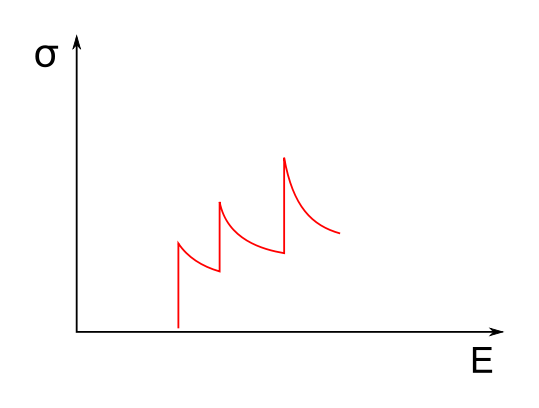
\includegraphics[width=.4\textwidth]{images/kante.png}
\caption{Schematischer Darstellung des Wirkungsquerschnittes als Funktion der Photonenenergie \cite{wikipedia}}
\label{fig:absorption}
\end{figure}

Die Sprungkanten werden als Absorptionskanten bezeichnet und sind im Absorptionsspektrum gut sichtbar. Der Photoeffekt ist also sehr wichtig bei kleineren Photonenenergien 
und Materialien mit hoher Kernladungszahl \cite{schatz}.

\subsection{Compton-Streuung}

Bei der Compton-Streuung wird nicht wie beim Photoeffekt die gesamte Energie auf eine Elektron übertragen, sondern nur ein Teil. Wie viel, hängt vom Winkel des 
Zusammenstoßes zwischen Photon und Elektron ab, es handelt sich also um einen elastischen Stoß. Das Elektron wird hierbei als frei angenommen, was bei den 
äußeren Elektronen eines Atoms näherungsweise stimmt. Durch den Energieverlust wird die Wellenlänge des Photons um den Betrag $\Delta \lambda$ vergrößert, für 
welche folgende Relation gilt:

\begin{align}
\Delta \lambda &= \frac{h}{m_e c} (1 - \cos \phi) = \lambda_c (1 - \cos \phi),
\end{align}
mit $\lambda_c$ der Compton-Wellenlänge, $m_e$ der Masse des Elektrons, $h$ dem Planckschen Wirkungsquantum, $c$ der Lichtgeschwindigkeit und $\phi$ dem Streuwinkel. 
Der Energieverlust hängt also allein vom Streuwinkel ab. 

Der Wirkungsquerschnitt ist somit allein von der Elektronendichte abhängig, welche ungefähr proportional zur Kernladungszahl ist. Somit ergibt sich für 
den Wirkungsquerschnitt folgende Näherung: 

\begin{align}
\sigma_C &\propto E_{\gamma}^{-1} \cdot Z
\end{align}

Der Comptoneffekt stellt sich somit aks besnders wichtig heraus für mittlere Energien zwischen $100$ und $1000 \si{\kilo \electronvolt}$. 

Wenn nun die gestreuten Photonen energieaufgelöst beobachtet werden, so ist die Energie des gestreuten Photons $E_{\gamma}'$ in Abhängigkeit des Winkel von Interesse:
\begin{align}
E_{\gamma}'(\phi) &= \frac{E_{\gamma}}{1 + \frac{E_{\gamma}}{m_e c^2} (1 - \cos \phi)}
\end{align}

Bei Aufnahme eines Spektrums ergibt sich nun also ein kontinuierliches Spektrum für alle Winkel zwischen 0\textdegree und 180\textdegree. Danach folgt eine 
scharfe Kante, die sogenannte Compton-Kante, die auftritt, weil nicht mehr Energie abgegeben werden kann, als bei einem Stoß von 180\textdegree. Die 
korrespondierende Energie beträgt dann also 
\begin{align}
E_{\gamma}'(180^{\circ}) &= \frac{E_{\gamma}}{1 + \frac{2 E_{\gamma}}{m_e c^2}}
\end{align}

Zusätzlich sollte ein Maximum mit höherer Energie im Spektrum auftreten, da auch einige Photonen ohne Streuprozess durch das Material fliegen. Dieses Maximum wird 
Photopeak genannt. Zu jedem Photopeak gibt es also eine korrespondierende Compton-Kante. 

\subsection{Paarbildung/-vernichtung}

Bei höheren Photonenenergien von ab $1022 \si{\kilo \electronvolt}$ tritt als zusätzlicher Effekt die Paarbildung bzw. -vernichtung auf. Hierbei kann sich ein Photon 
im Feld eines Atoms in Elektron und Positron aufspalten. 


\subsection{Massenschwächungskoeffizient}

\begin{figure}[h]
\centering
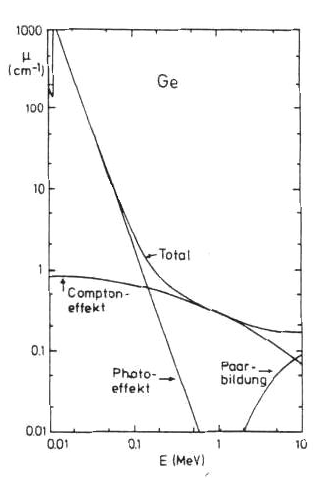
\includegraphics[width=.4\textwidth]{images/absorption.pdf}
\caption{Beitrag der verschiedenen Komponenten zum Absorptionskoeffizienten von Germanium \cite{schatz}}
\label{fig:absorption_2}
\end{figure}

\subsection{Szintillationsdetektor}

Der moderne Szintillationsdetektor oder -zähler beseht aus zwei Teilen: Dem Szintillator und dem Photomultiplier. Im Szintillator werden durch ionisierende Strahlung 
Exzitonen erzeugt. Diese ionisieren weitere Atome im Gitter. Energiereiche Strahlung erzeugt also mehrere Elektron-Loch-Paare. Diese rekombinieren nun wieder. 
Findet dies an den dotierten Störstellen statt, wird Energie in Form von Lichtblitzen frei \cite{kleinknecht}. Diese können mithilfe eines Photomultipliers 
festgestellt werden. Das Signal ist dann proportional zur Energie der detektierten Strahlung. Damit die Lichtblitze detektiert werden können, muss das Detektormaterial 
für sichtbares Licht durchsichtig sein. Daher ist der Szintillator 
häufig als Einkristall ausgeführt. Im Experiment wird als Material ein Thallium dotierter Natrium-Iodid Kristall verwendet. Das Thallium nimmt dabei den Platz der 
Natrium-Positionen im kubischen Kristallgitter ein. Je nach Dotierungskonzentration ändert sich die Auflösung des Detektors. 

\subsection{Halbleiterdetektor}

Ein Halbleiterdetektor besteht meist aus einem p-n-Übergang, bei dem ein positiv und ein negativ dotierter Halbleiter, in diesem Fall Germanium, aneinandergebracht werden. 
Fällt nun Strahlung in den Halbleiter ein, so erzeugt diese Elektron-Loch-Paare. Dies geschieht analog zum Szintillator durch anregung eines einzelnen Elektrons, 
welches dann auf seiner Bahn durch den Halbleiter weitere Elektronen anregt. Diese können abgegriffen und der erzeugte Strom oder die Schwankung in der Spannung gemessen 
werden. Die Anzahl der freigesetzten Elektronen wird dabei durch die Bandlücke bestimmt, da diese Energie zum anheben in das Leitungsband benötigt wird. Da diese 
Bandlücke nicht sehr groß ist, kann die Energie der Strahlung sehr gut aufgelöst werden. Um möglichst alle angeregten 
Elektronen abfangen zu können, wird eine Hochspannung angelegt, die die Elektronen absaugt und die Sperrschicht vergrößert. Außerdem wird der Detektor gekühlt, um 
eine thermische Anregung ins Leitungsband zu verhindern und um den Leckstrom gering zu halten, der bei der angelegten Hochspannung den Detektor zerstören kann 
\cite{nicoletti}. 

Als Detektormaterial wird ein Halbleiter mit hoher Kernladungszahl verwendet, in diesem Fall Germanium, da diese einen höheren Wirkungsquerschnitt aufgrund der höheren 
Elektronenzahl aufweisen.

Normalerweise beträgt die statistische Schwankung von $n$ Messwerten $\sigma_n = \sqrt{n}$. Durch die Fanoresonanz wird diese jedoch reduziert, sodass hier 
$\sigma_n = \sqrt{n F}$ gilt, wobei $F$ den Fano-Faktor beschreibt. Dieser kann bei Germanium im auf Werte bis zu $F \approx 0,13$ schrumpfen \cite{fano}. 
Diese Reduzierung des statistischen Fehlers ist darauf zurückzuführen, dass die Energieverluste in inelastischen Streuprozessen im Festkörper nicht komplett zufällig 
verlaufen, sondern durch die Beträge der möglichen Übergänge aus den Elektronenschalen limitiert sind.

\section{Durchführung}

\subsection{Versuchsaufbau}

\begin{figure*}[h]
\centering
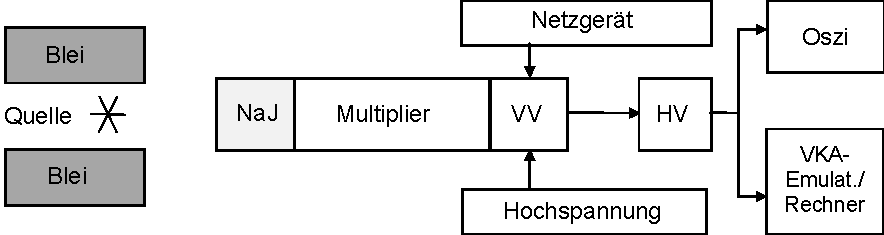
\includegraphics[width=.8\textwidth]{images/aufbau.pdf}
\caption{Schematischer Aufbau des Versuchs \cite{wiki} mit NaJ-Detektor, VV-Vorverstärker, HV-Hauptverstärker, VKA-Vielkanalanalysator}
\label{fig:aufbau}
\end{figure*}

\subsection{Ablauf}

\section{Auswertung}


\newpage
\bibliographystyle{unsrtnat}
\bibliography{gammabib}

\end{document}





